\section{Result}

The simulated events and g12 data are passed all selection and cuts described in  Section.~\ref{Cor}, Section.~\ref{VCut}, Section.~\ref{TCut}, Section.~\ref{Cos} and Section.~\ref{KF}. The number of the events rejected in both the simulation and data after the cuts is shown in a Table.~\ref{tab3}. 
  
\begin{table}[]
\centering
\begin{tabular}{|c|c|c|}
\hline
Cuts                                        & g12 Run 56655                    & Simulation \\
\hline
Generated                               & ---                          & 10001500   \\
Reconstructed                           & 42947                        & 855447     \\
Vertex Cut                              & 20092                        & 505405     \\
Timing Cut                              & 11390                        & 451470     \\
Multiple $E_{\gamma}$ & 14986 & ---            \\
Fiducial Cuts                           & 10541                        & 276432     \\
Prob(($\eta$)$\pi^{+}$$\pi^{-}$p) \textgreater 0.01                & 1901                         & 259136    \\
\hline
\end{tabular}
\caption{The table shows the cut flow of the analysis from g12 data run 56655 and simulated events.}
\label{tab3}
\end{table}
 
 In an attempt to see how well the simulation explains the g12 data a comparison of the kinematic variables of the center-of-mass energy ($\sqrt{s}$) and momentum (P), $\theta$ and $\phi$ for $\pi^{+}$ $\pi^{-}$ and p is shown in the Figure.~\ref{fig6}, ~\ref{fig7}, ~\ref{fig8} $\&$ ~\ref{fig9}. The events in the Monte Carlo are generated with the model explained in Section.~\ref{Sim} with the input Dalitz plot parameters from BESIII measurement~\cite{Ablikim:2010kp}.

\begin{figure}[ht!]
\centerline{
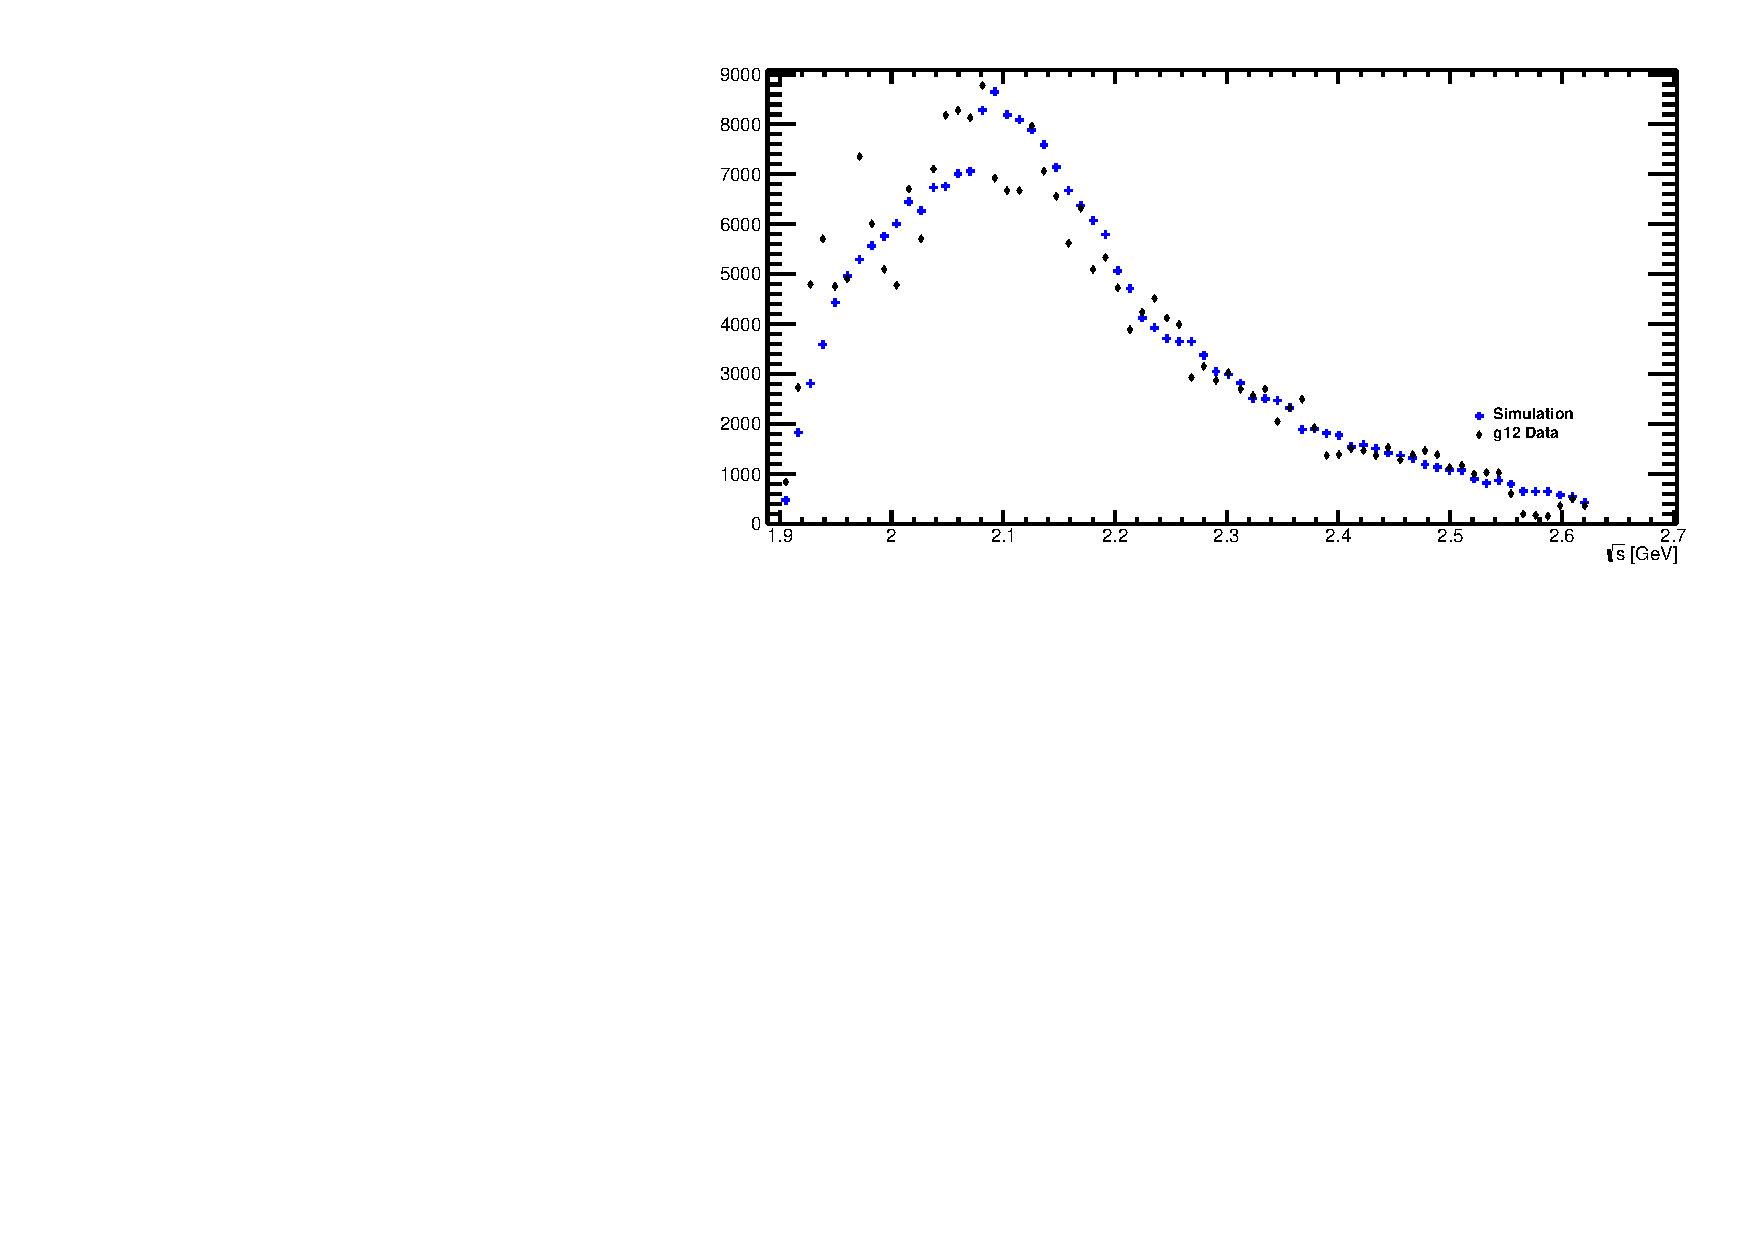
\includegraphics[width=10cm,height=6cm]{w.pdf}}
\caption{Comparison of incident photon beam in center of mass energy ($\sqrt{s}$) with simulated (blue) events and g12 data (black) when generating Monte-Carlo with the differential cross-sections and Dalitz plot parameters.}
\label{fig6}
\end{figure}

\begin{figure}[ht!]
\centerline{
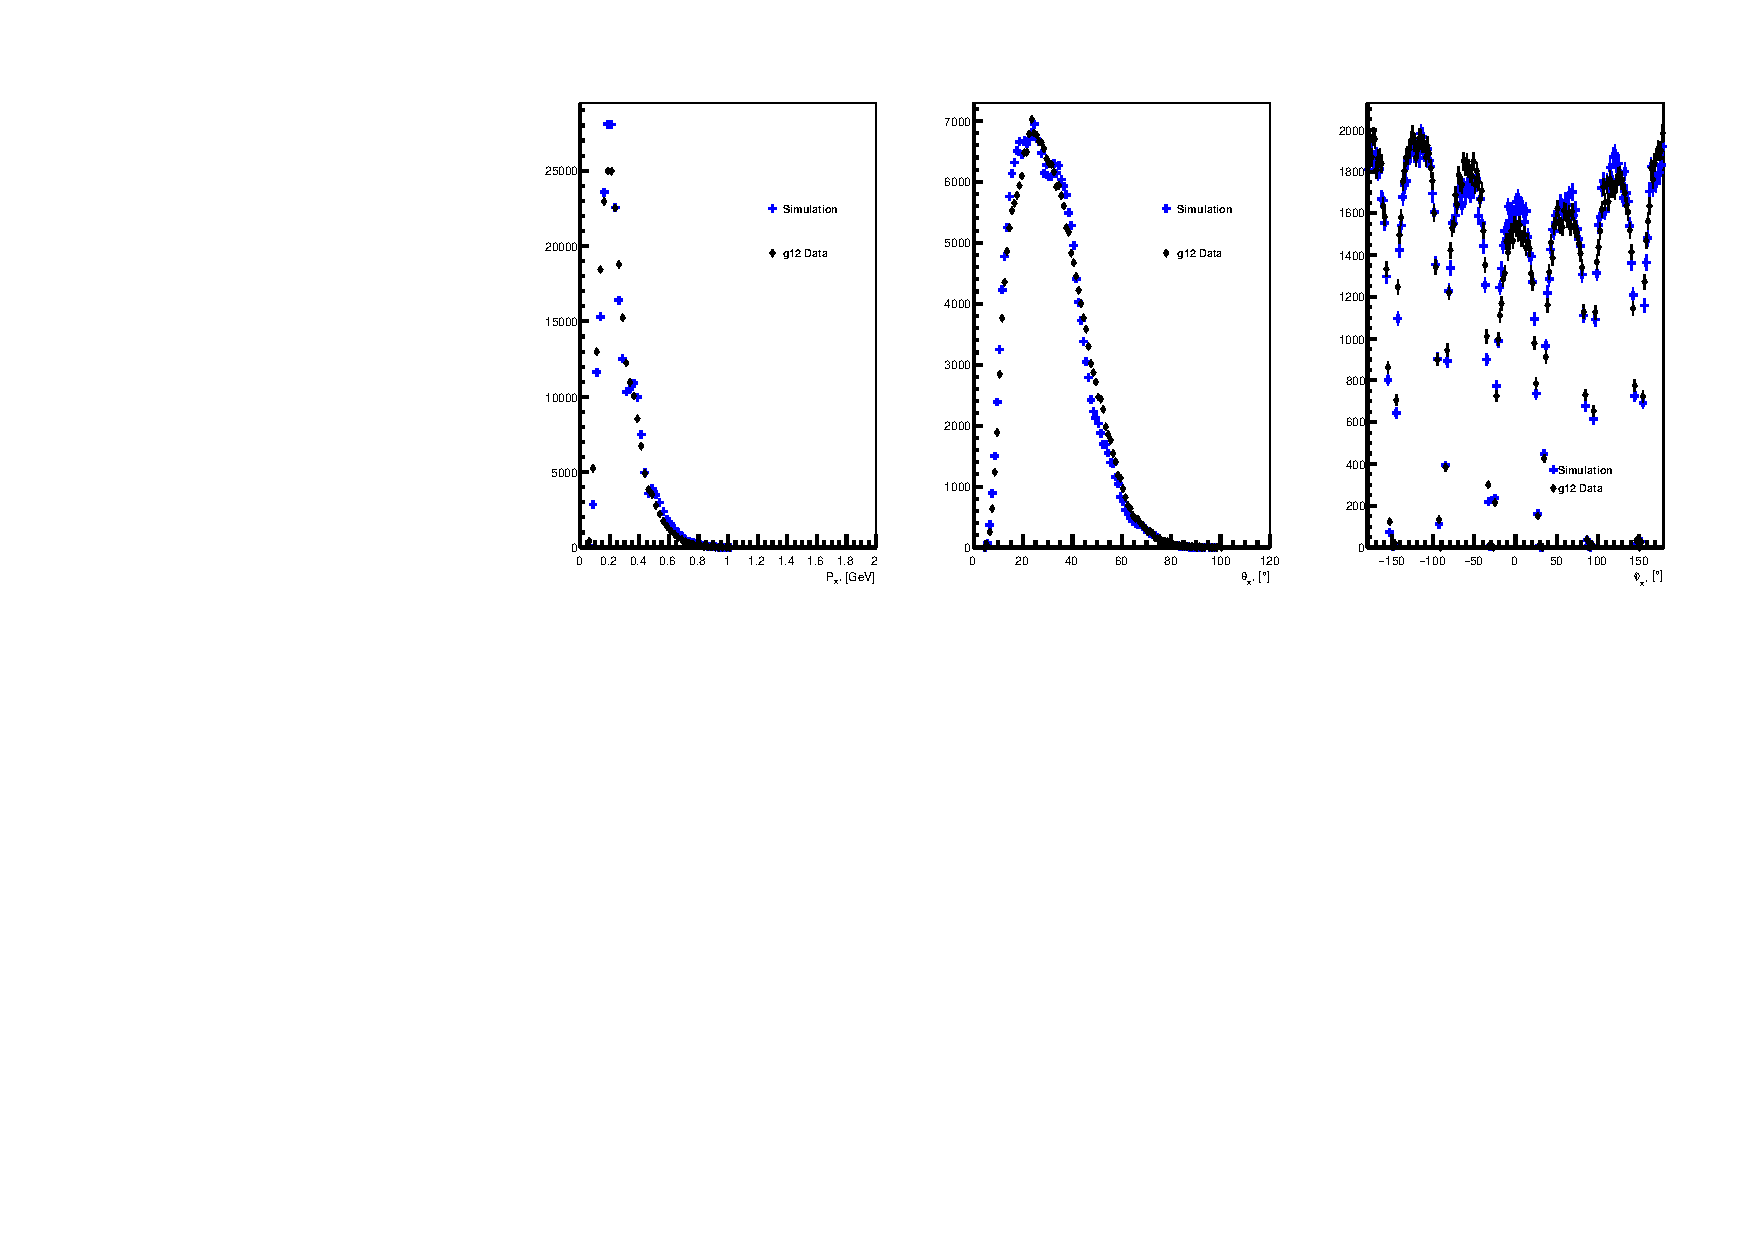
\includegraphics[width=14cm,height=4cm]{Pip.pdf}}
\caption{Comparison of  $\pi^{+}$ momentum (left), $\pi^{+}$ $\theta$ (middle) and $\pi^{+}$ $\phi$ (right) with simulated (blue) events and g12 data (black) when generating Monte-Carlo with the differential cross-sections and Dalitz plot parameters.}
\label{fig7}
\end{figure}
 
\begin{figure}[ht!]
\centerline{
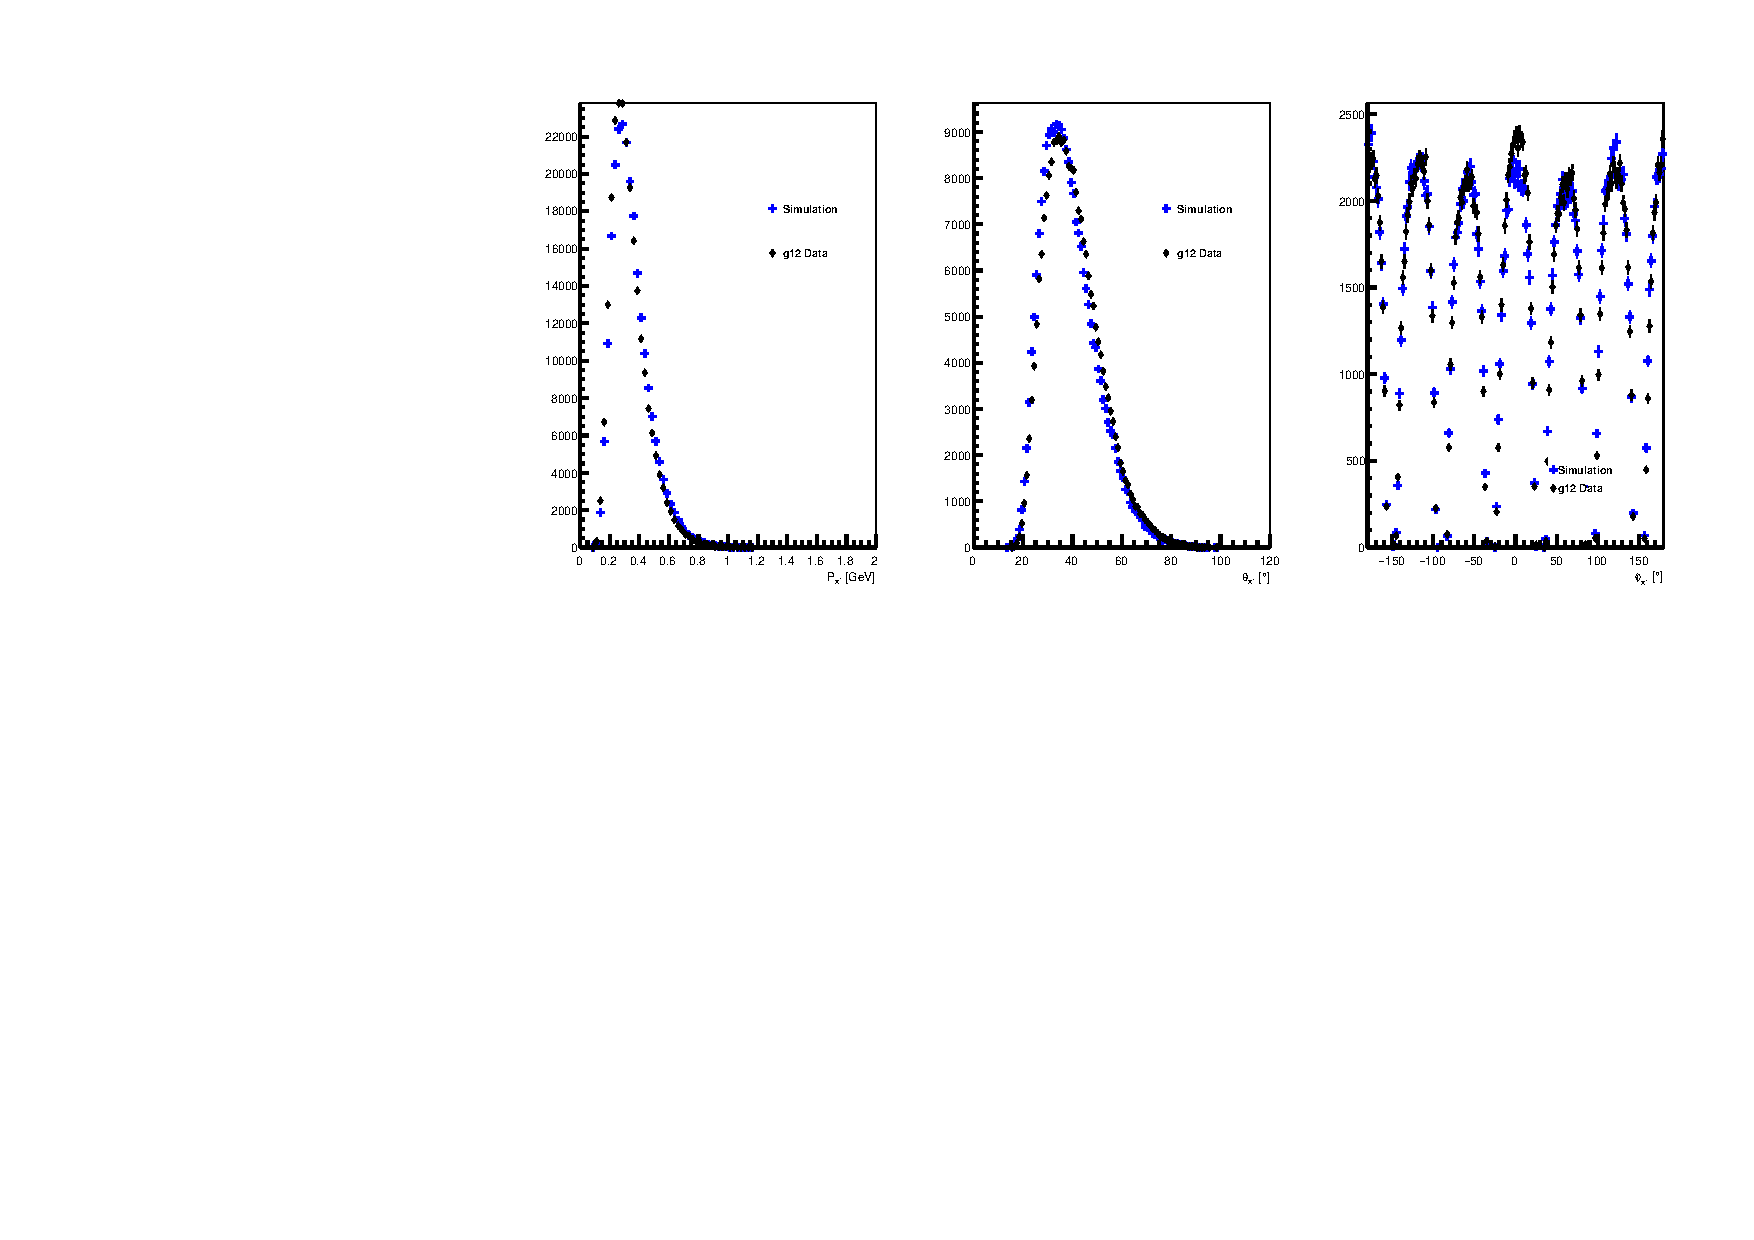
\includegraphics[width=14cm,height=4cm]{Pim.pdf}}
\caption{Comparison of $\pi^{-}$ momentum (left), $\pi^{-}$ $\theta$ (middle) and $\pi^{-}$ $\phi$ (right) with simulated (blue) events and g12 data (black) when generating Monte-Carlo with the differential cross-sections and Dalitz plot parameters.}
\label{fig8}
\end{figure}

\begin{figure}[ht!]
\centerline{
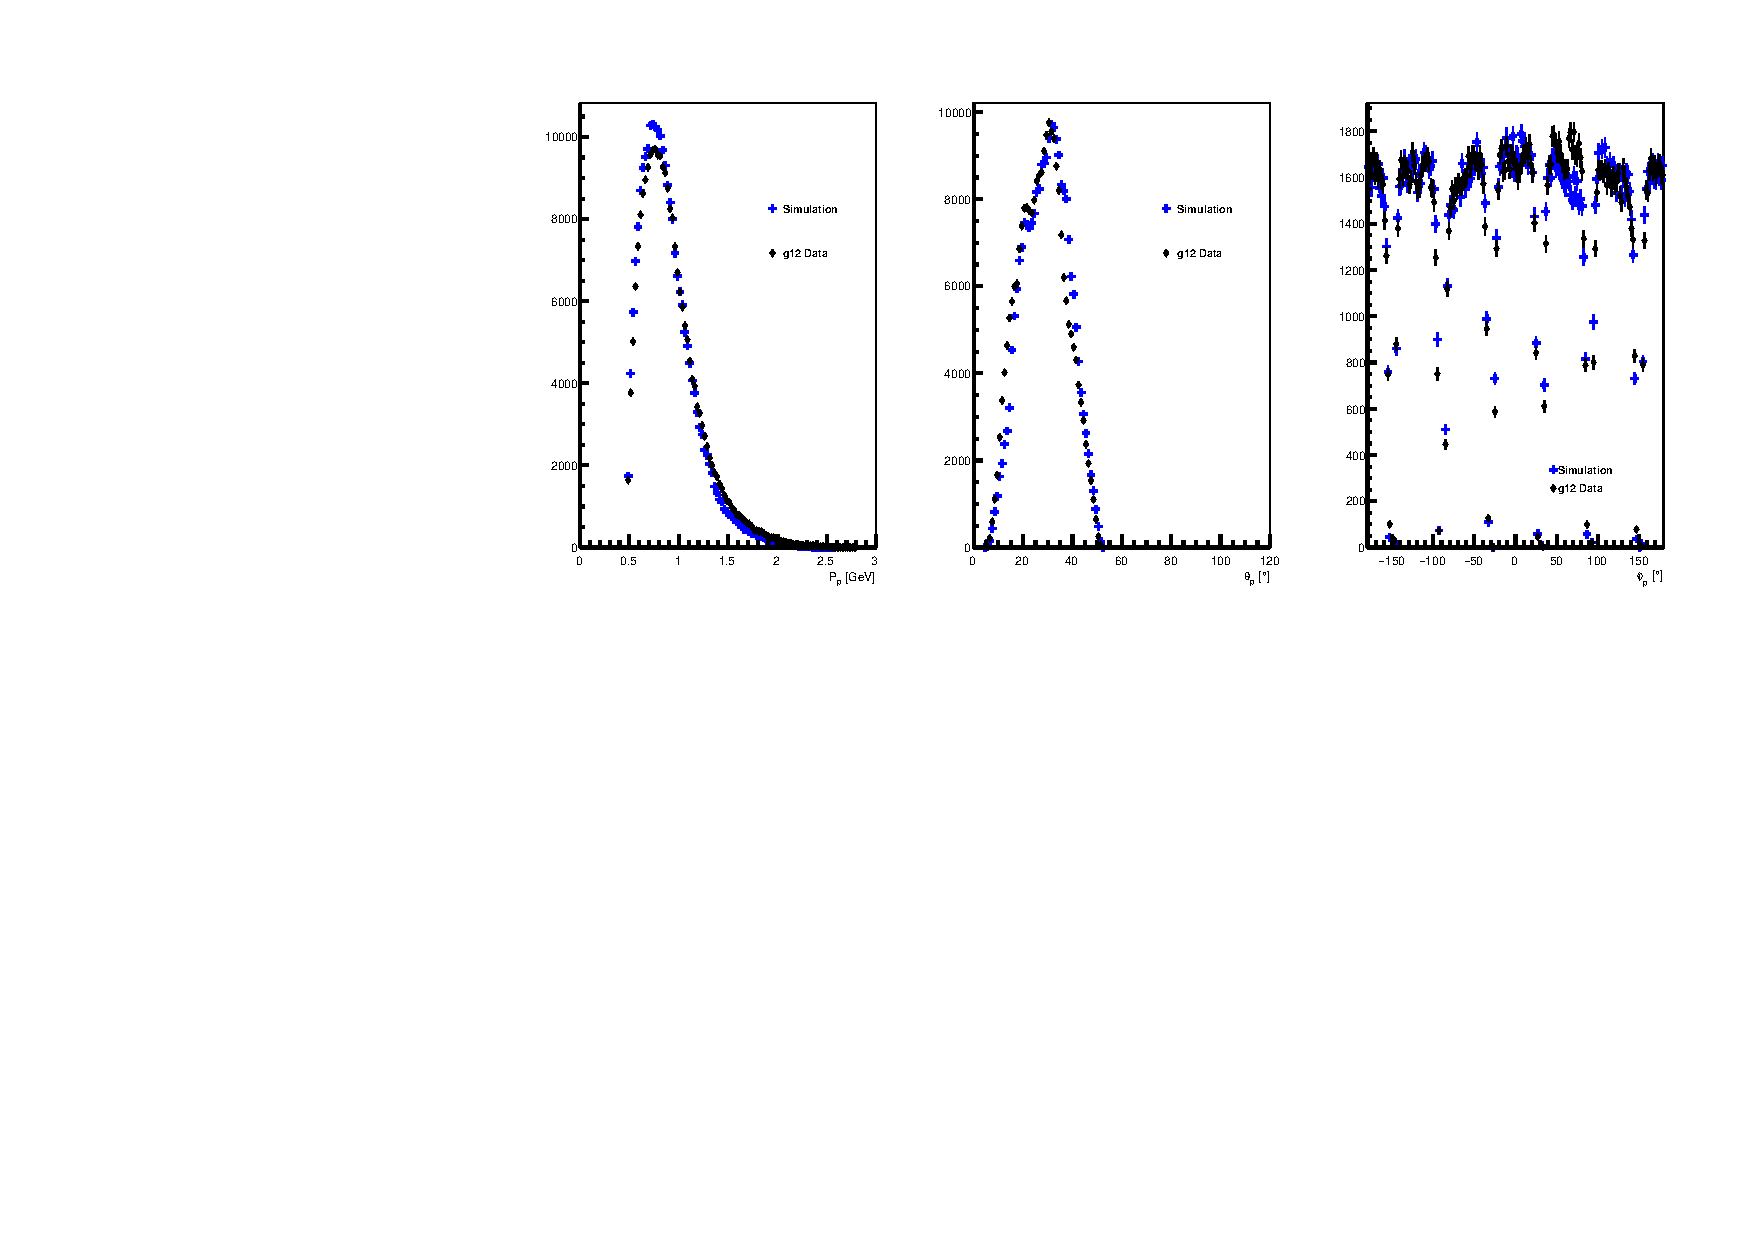
\includegraphics[width=14cm,height=4cm]{P.pdf}}
\caption{Comparison of proton momentum (left), proton $\theta$ (middle) and proton $\phi$ (right) with simulated (blue) events and g12 data (black) when generating Monte-Carlo with the differential cross-sections and Dalitz plot parameters.}
\label{fig9}
\end{figure}
 
 
 \subsection{Background subtraction to the Dalitz plot}

\begin{figure}[ht!]
\centerline{
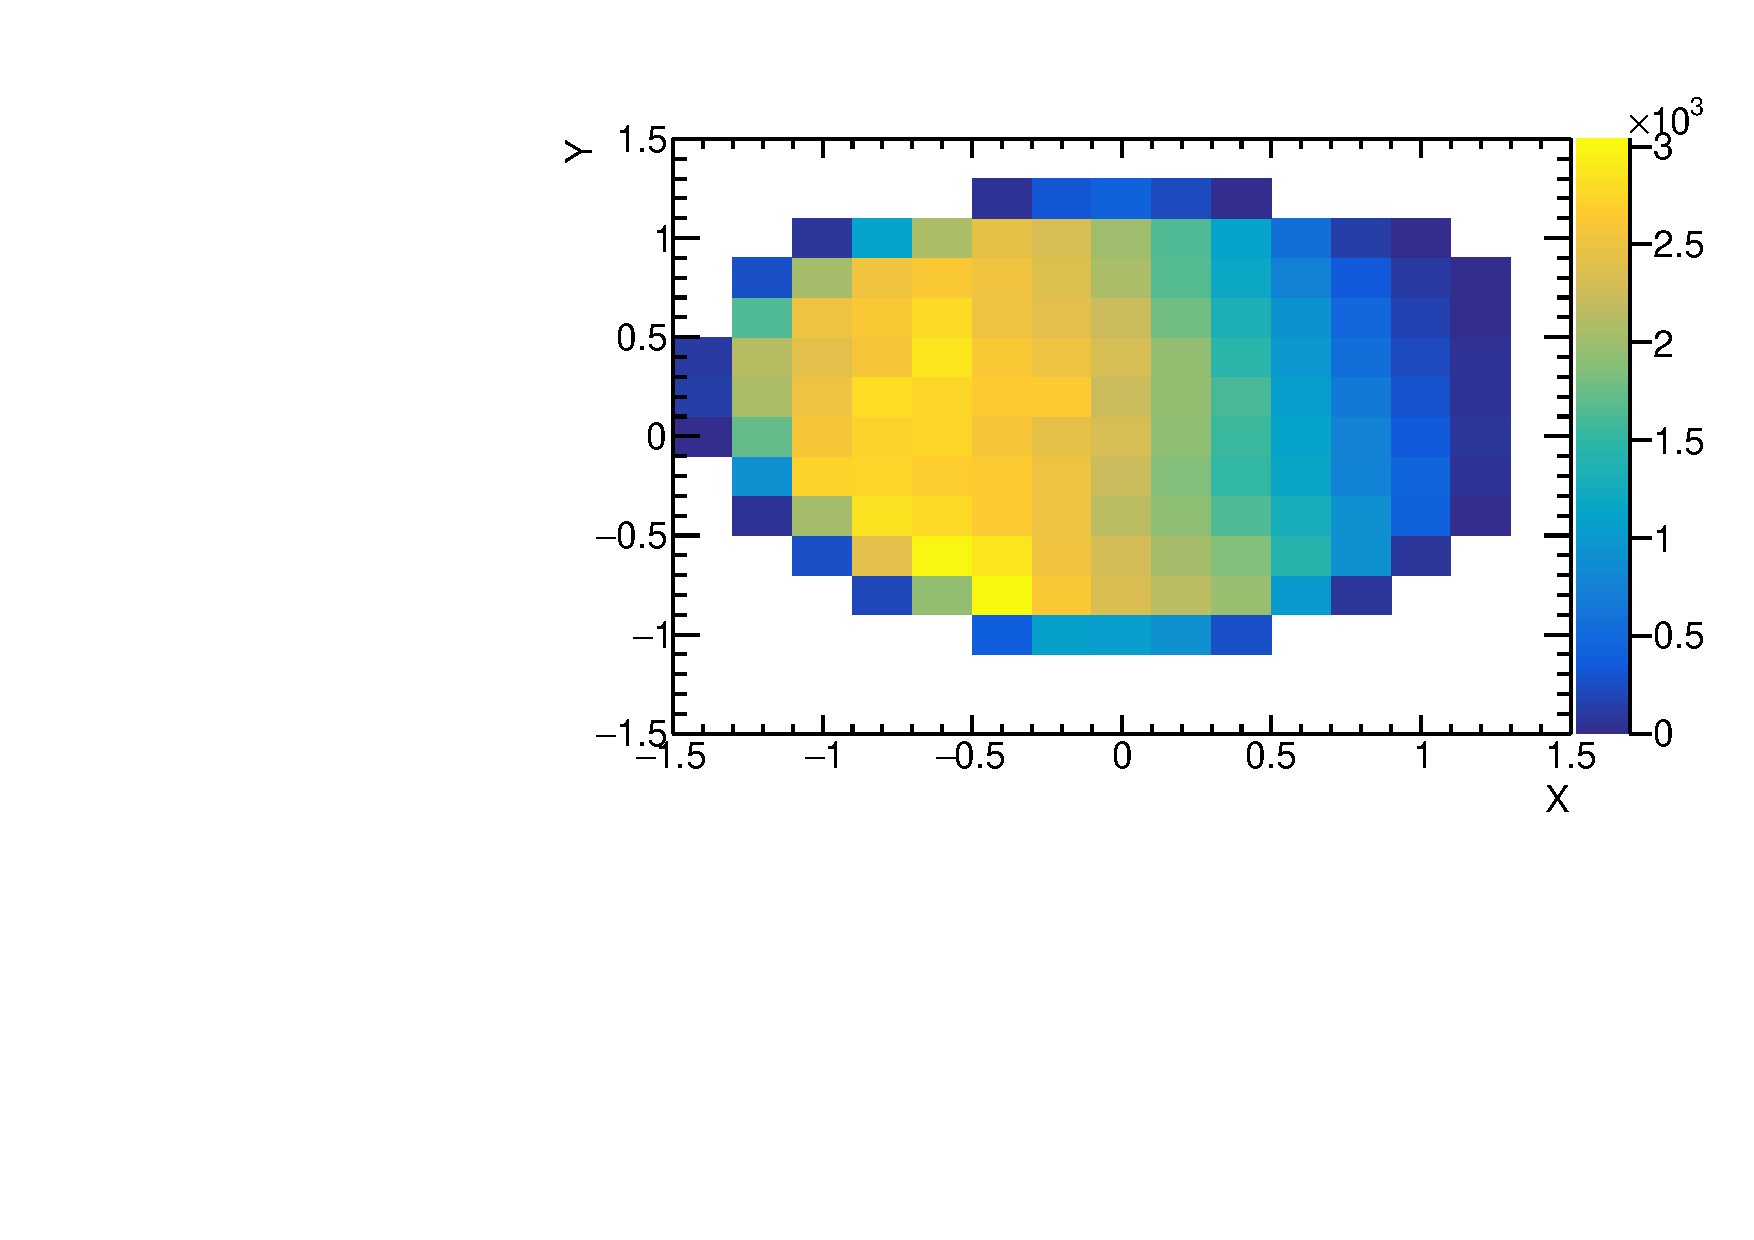
\includegraphics[width=10cm,height=6cm]{Before_BS.pdf}}
\caption{Dalitz plot before background subtraction.}
\label{B4_DP}
\end{figure}

The aim is to obtain a bin-wise background subtracted Dalitz plot. In order to achieve that all the events are feed into a X and Y (nbin x nbin) Dalitz plot and a bin-wise background subtraction is performed to the $M_{x}$(p) distribution after restricting 0.537 $\leq$ $M_{x}$(p$\pi{+}$$\pi{-}$) $\leq$ 0.557. The signal in $M_{x}$(p) distribution is fitted with a Voigt function and background is fitted with a Polynomial of order 3 in each bin of the Dalitz plot to subtract the non-resonant contribution. The fit to a low and high statistics bin shown in Figure.~\ref{DP_fit}. The events under the background subtracted 3 standard deviation region is the number of events in the Dalitz plot bin. The number of events in each Dalitz plot bin has ``$N_{i}$" events and the error is ``$\sigma_{i}$", given by 
\begin{equation}
\sigma = \sqrt{S_{1} + (S+B - S_{1})}
\end{equation}
where ``i" goes from 1 to total number of bins in the Dalitz plot. $S_{1}$ is the background subtracted peak and S+B is the total number of events in the $M_{x}$(p) spectrum in the 3 standard deviation.

\begin{figure}[ht!]
\centerline{
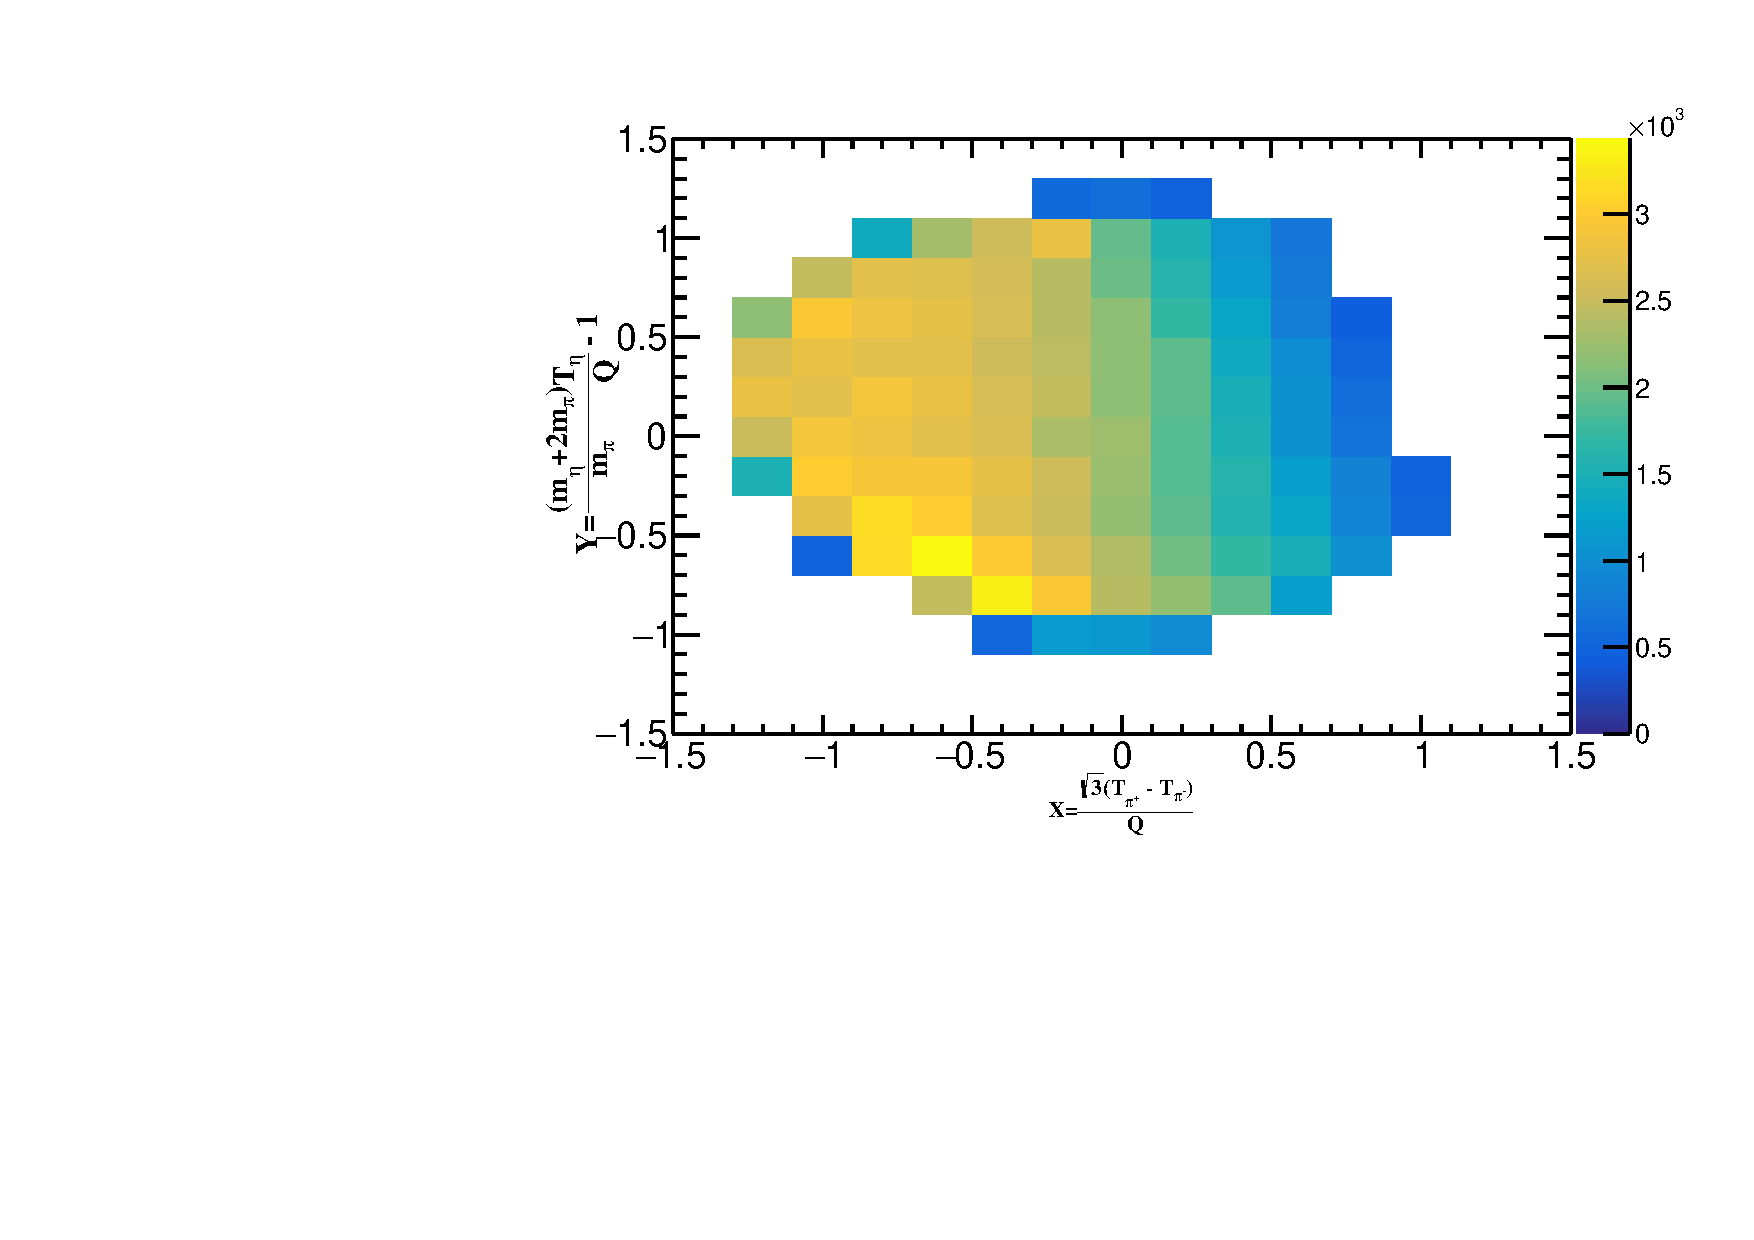
\includegraphics[width=10cm,height=6cm]{After_BS.pdf}}
\caption{Dalitz plot after background subtraction.}
\label{Af_DP}
\end{figure}

\begin{figure}
\centering
\begin{subfigure}{.5\textwidth}
  \centering
  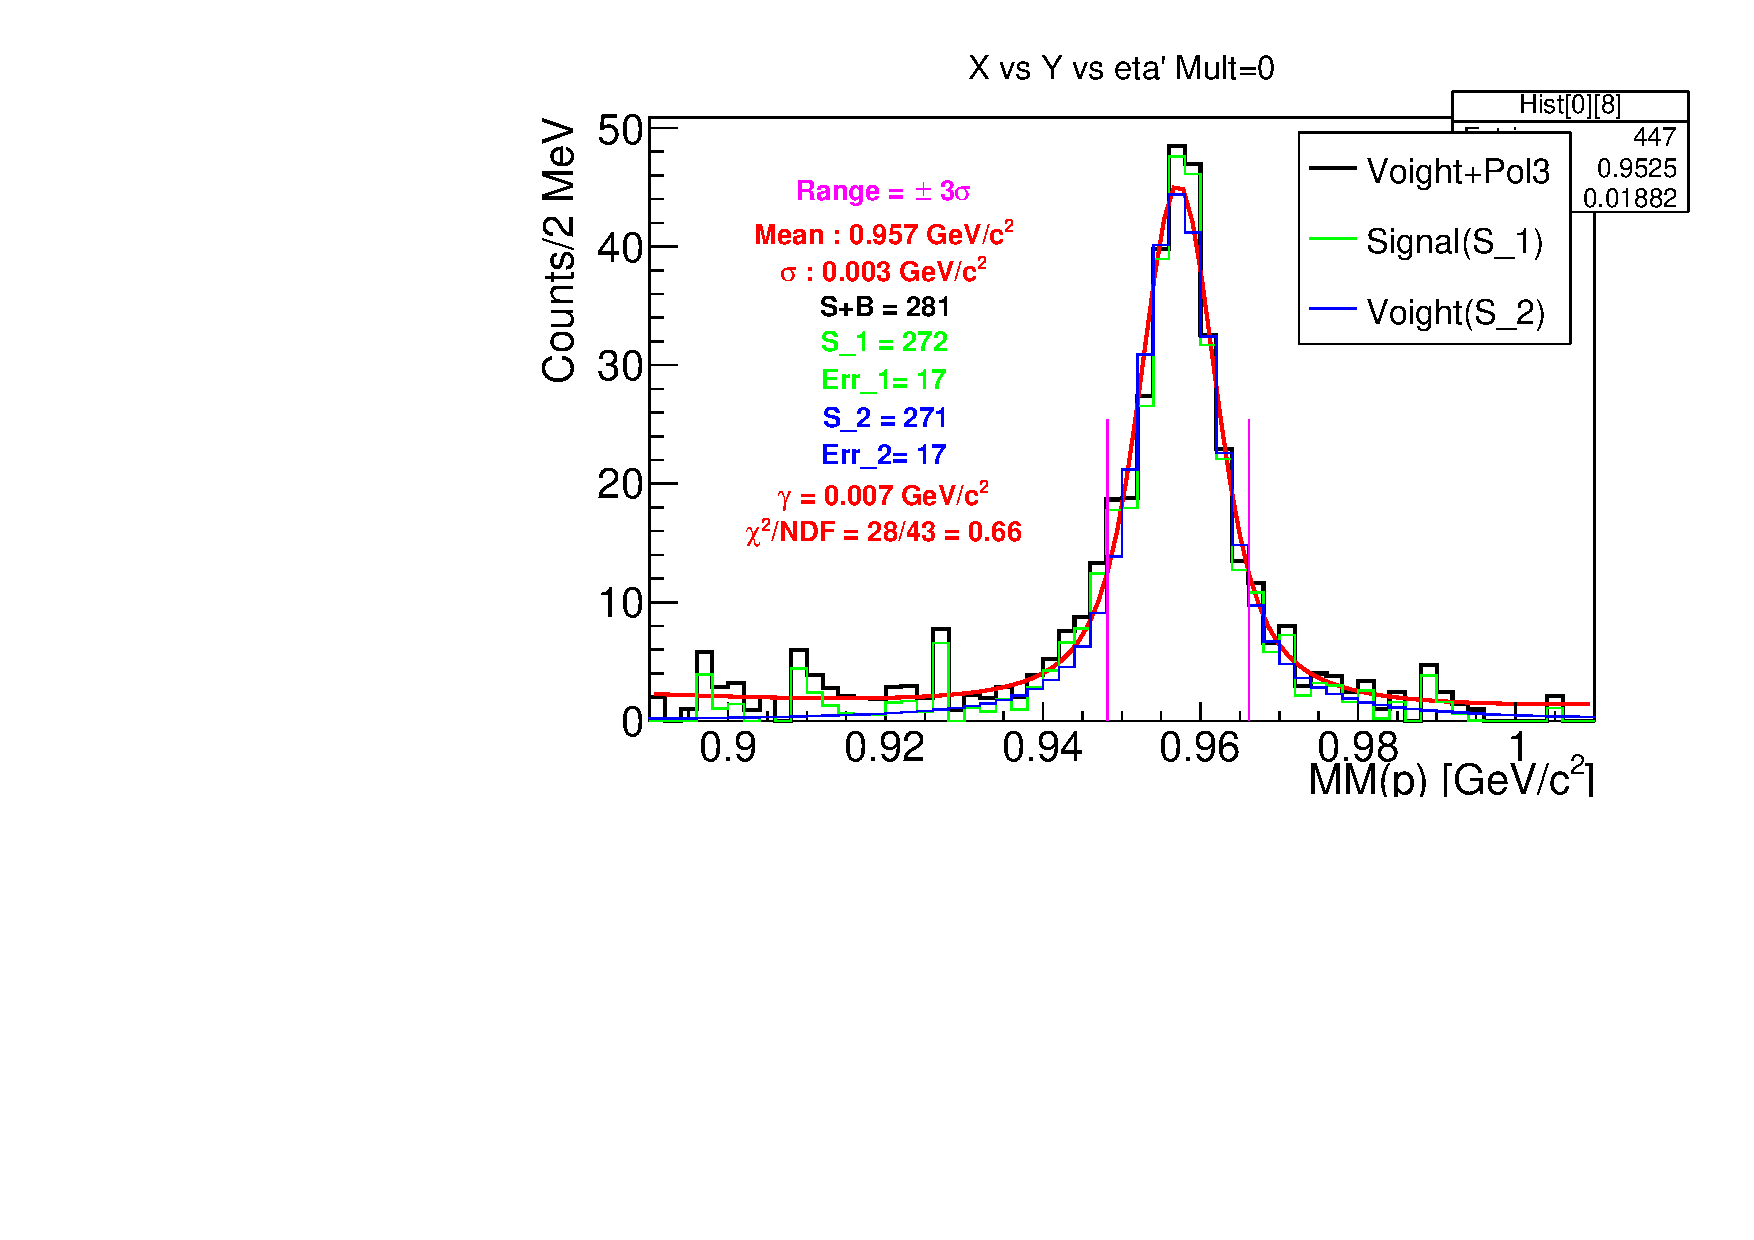
\includegraphics[width=.7\linewidth]{Hist[0][8].pdf}
  \caption{Fit to the $M_{x}$(p) distribution to a low statistics bin of Dalitz plot.}
  \label{fig:sub1}
\end{subfigure}%
\begin{subfigure}{.5\textwidth}
  \centering
  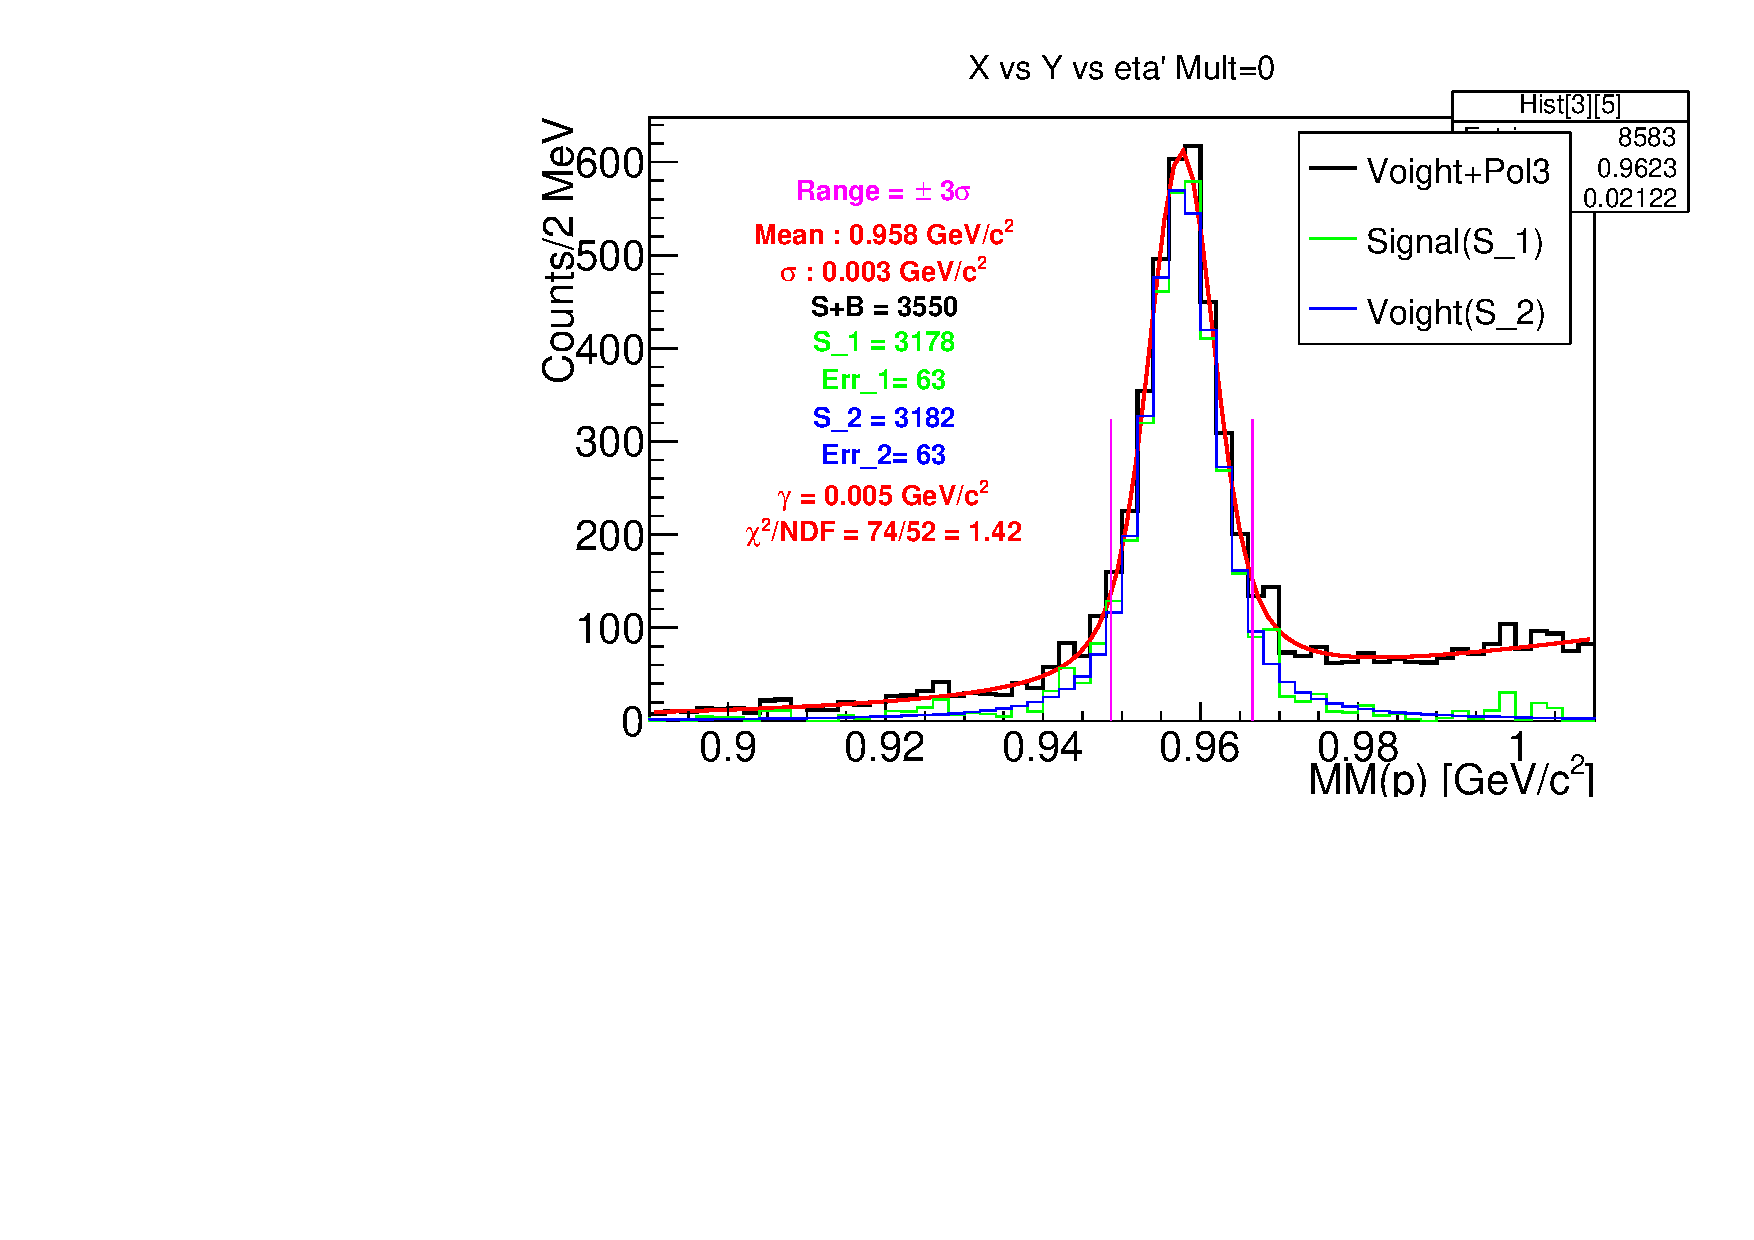
\includegraphics[width=.7\linewidth]{Hist[3][5].pdf}
  \caption{Fit to the $M_{x}$(p) distribution to a higher statistics bin of Dalitz plot.}
  \label{fig:sub2}
\end{subfigure}
\caption{A figure with two subfigures}
\label{DP_fit}
\end{figure}




One can also define the boundary of the $\eta^{\prime}$ $\rightarrow$ $\eta$ $\pi^{+}$ $\pi^{-}$ decay from the fact that the addition three momenta of particles $\vec{P}_{\eta}$, $\vec{P}_{\pi+}$ and $\vec{P}_{\pi-}$ for $\eta$, $\pi^{+}$ and $\pi^{-}$ respectively is 0 in the rest frame of $\eta^{\prime}$.
\begin{eqnarray*}
\vec{P}_{\eta} + \vec{P}_{\pi+} + \vec{P}_{\pi-} = 0.
\end{eqnarray*}
Squaring and equating the side gives us the boundary Equation.~\ref{bd} of the $\eta^{\prime}$ $\rightarrow$ $\eta$ $\pi^{+}$ $\pi^{-}$ decay.
\begin{eqnarray}
|{{P}_{\eta}}^2 - {{P}_{\pi+}}^2 - {{P}_{\pi-}}^2| \leq 2\vec{P}_{\pi+} . \vec{P}_{\pi-}
\label{bd}
\end{eqnarray}

One can also translate the 2D Dalitz plot bins of X and Y with a global bin number given by:
\begin{eqnarray*}
Globalbin(X,Y) = 
Floor \big[ \frac{X + X_{max}}{\delta} \big] + N_{bins} . Floor \big[ \frac{Y + Y_{max}}{\delta} \big] + 1
\label{gb}
\end{eqnarray*}
where X and Y are the central values of the current bin, $X_{max}$ and $Y_{max}$ are the maximum values the axis X and Y respectively, which is chosen to be 1.5. The $N_{bins}$ are the number of bins chosen along X and Y axis and it is 15 here. A translation of the Dalitz plot to its Global bin number along with the boundary of the decay from Equation.~\ref{bd} is shown in Figure.~\ref{fig10}. A global bin translation of the background subtracted Dalitz plot is shown in Figure.~\ref{DP_gl}.

\begin{figure}[ht!]
\centerline{
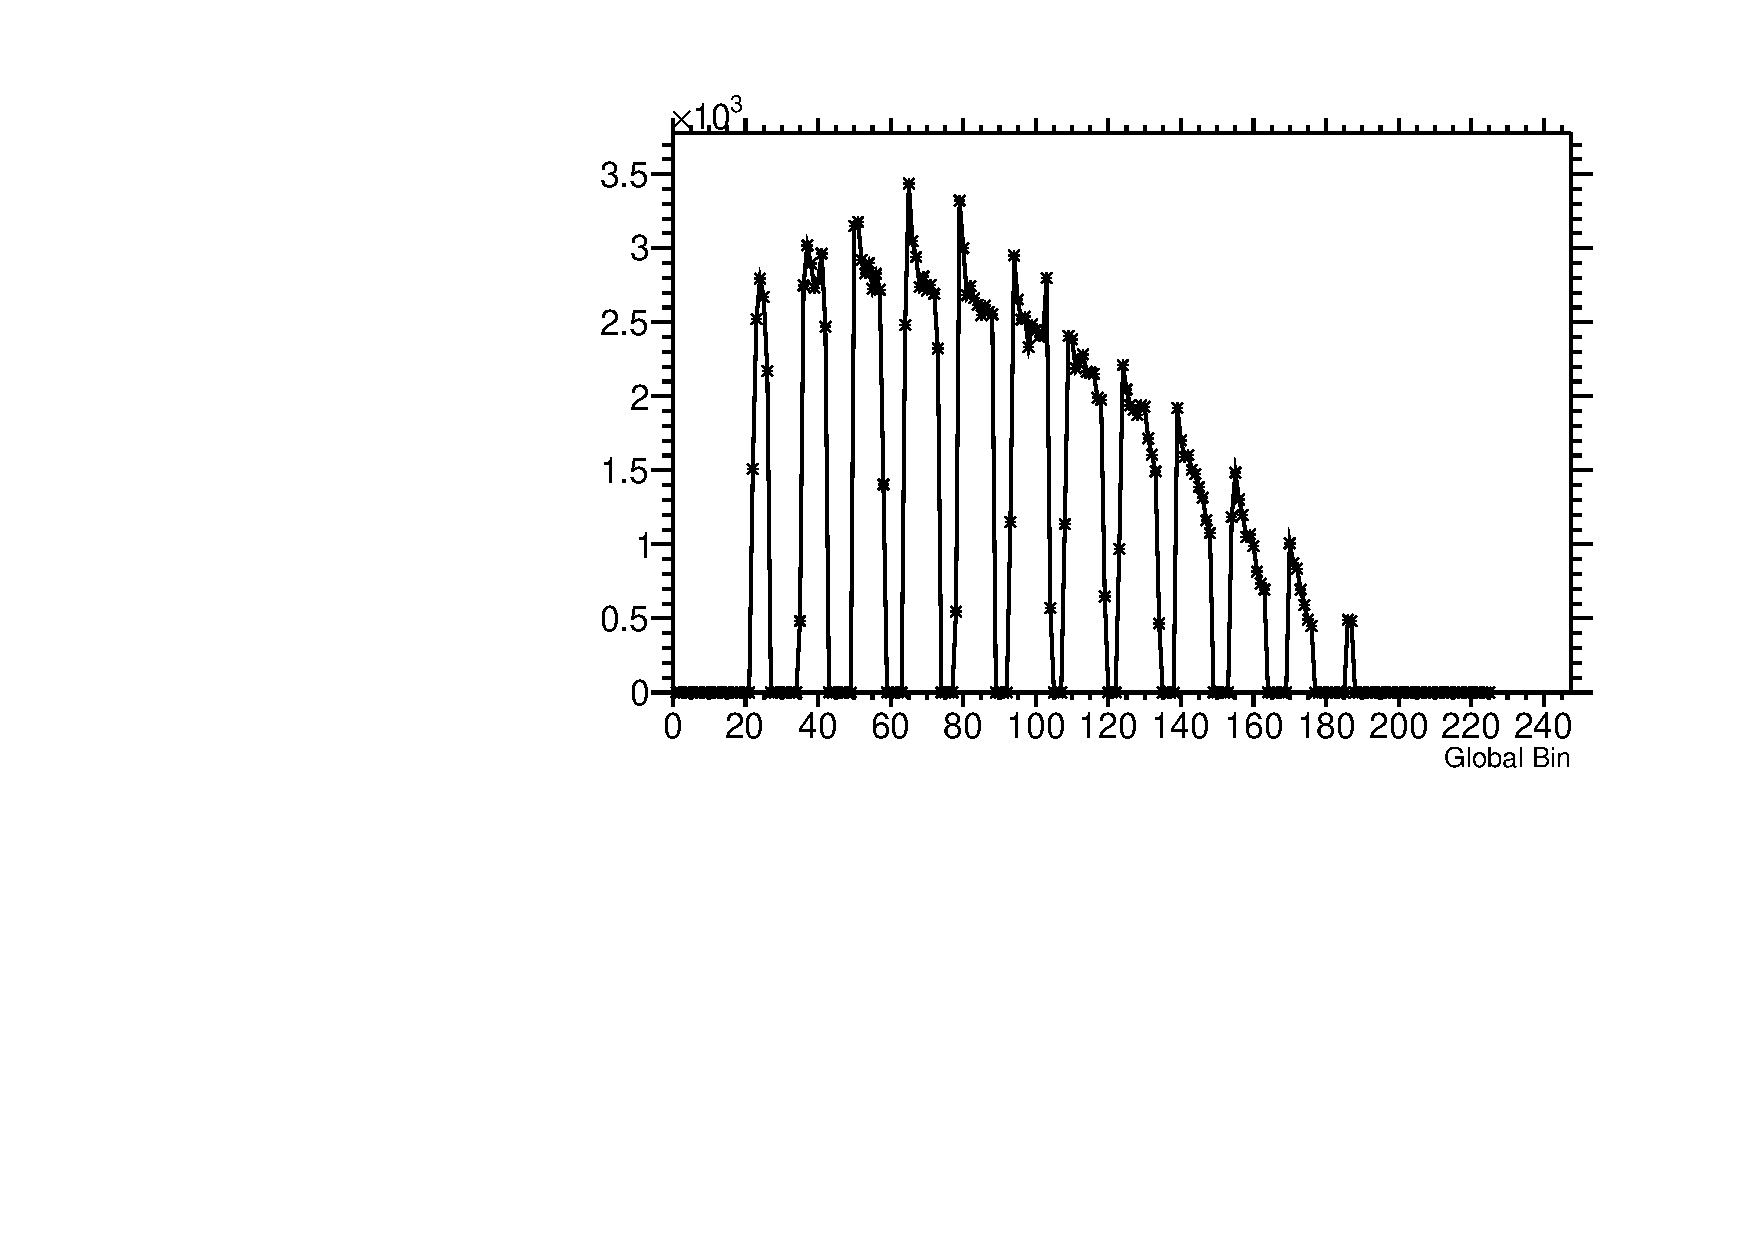
\includegraphics[width=10cm,height=6cm]{DP_Global.pdf}}
\caption{The background subtracted Dalitz plot in global bins.}
\label{DP_gl}
\end{figure}
 

%FIGURE OF DP WITH GLOBAL BIN
%FIGURE OF DATA DP WITH GLOBAL BIN
 
\begin{figure}[ht!]
\centerline{
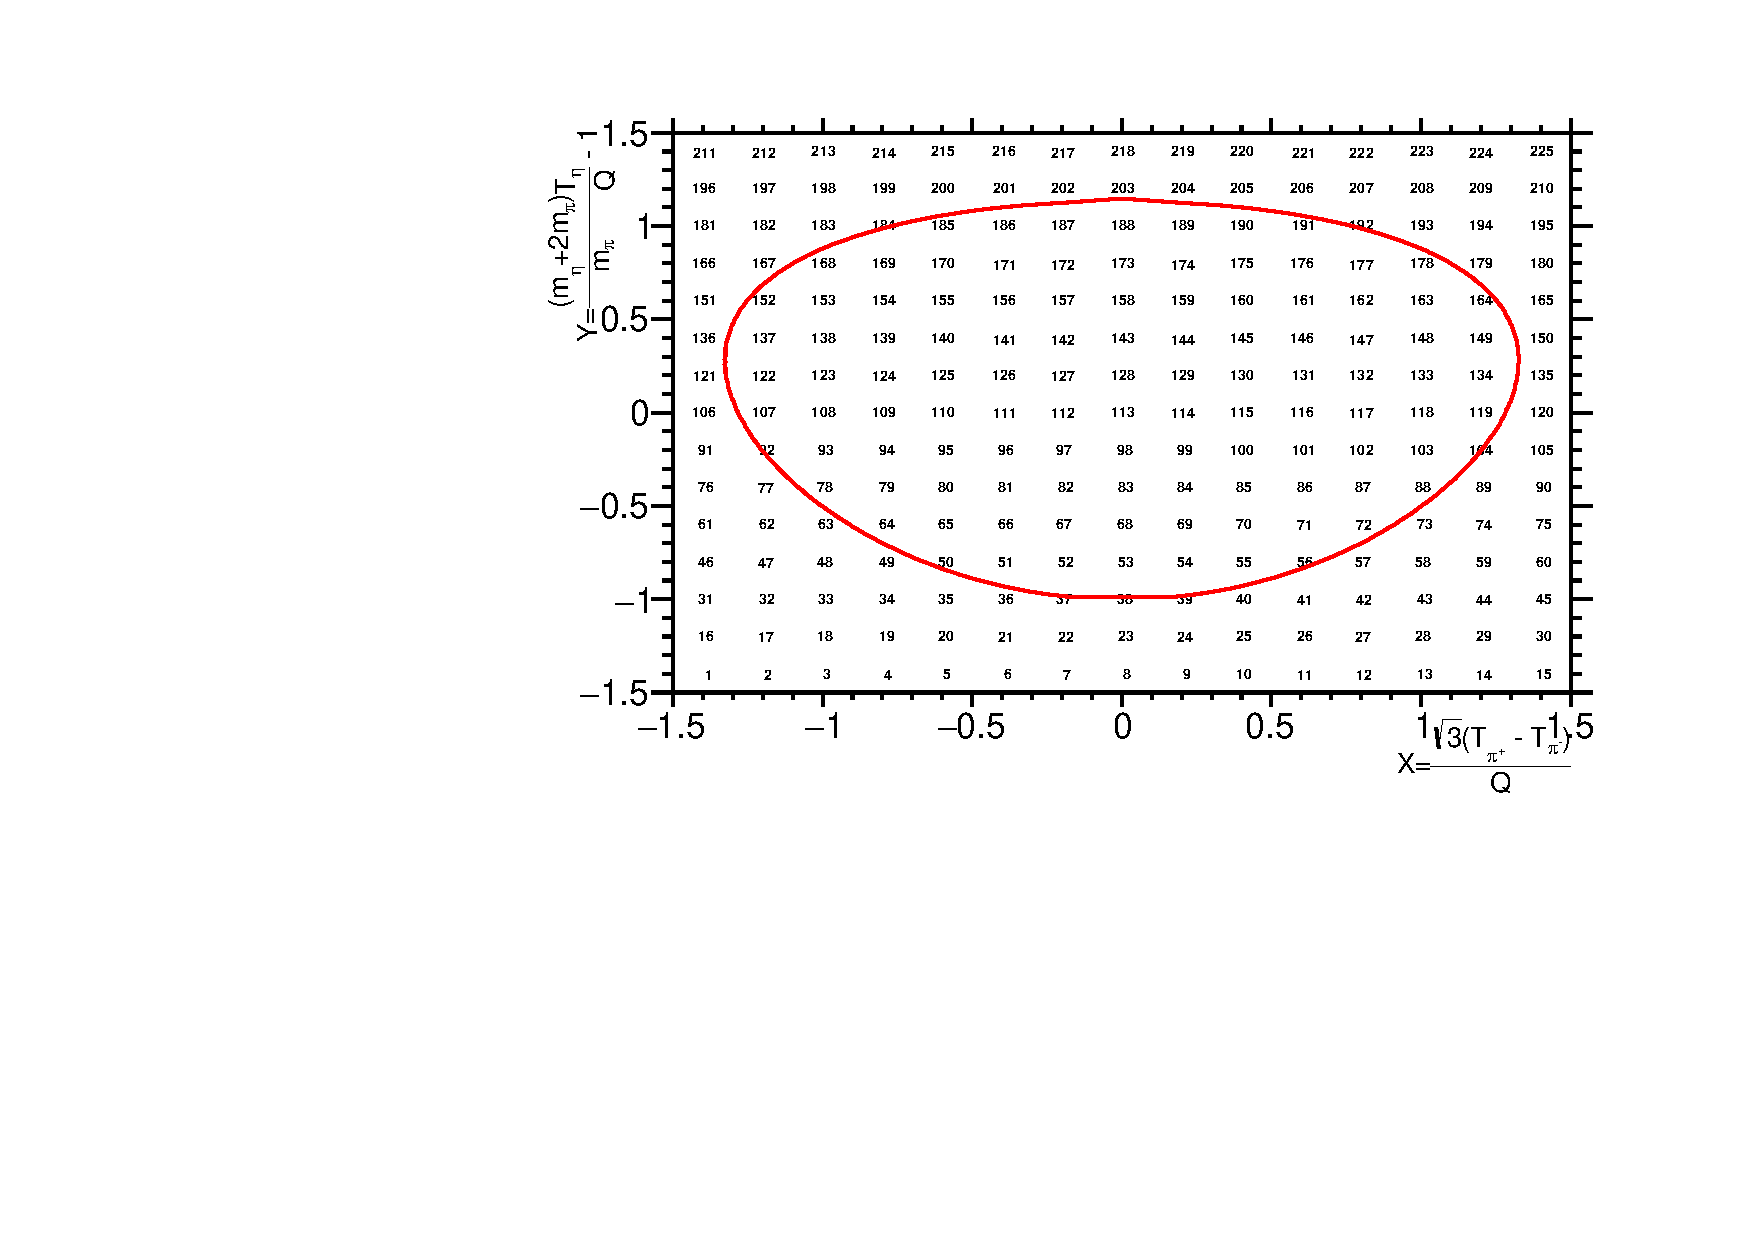
\includegraphics[width=14cm,height=8cm]{gb.pdf}}
\caption{The 15 x 15 Dalitz plot shows the translation X and Y Dalitz plot bins in global binning and the red curve shows the phase space boundary of the decay. }
\label{fig10}
\end{figure} 

 %FIGURE WITH 1D DP

\subsection{Calculation of acceptance with smearing matrix}

The CLAS detector has a different acceptance of proton, $\pi^{+}$ and $\pi^{-}$ and the acceptance varies within the phasespace of the  $\eta^{\prime}$ $\rightarrow$ $\eta$ $\pi^{+}$ $\pi^{-}$ decay. Hence the migration of events in different bins within the phasespace is also non-uniform, so one must take special care of migration of events from one bin to the other. To take care of the migration of the events,  an acceptance with smearing matrix ($\epsilon_{n,m}$) is presented here. The events are generated in each bin of the Dalitz plot and the acceptance for all the bins including the migrated bins are calculated. For events generated in the $j^{th}$ bin, the acceptance is calculated for all $i^{th}$ Dalitz plot bins as shown below :
\begin{eqnarray}
\epsilon_{i,j} = \frac{N_{rec,gen}(i,j)}{N_{gen}(j)}
\end{eqnarray}
Where $N_{rec,gen}$(i,j) denotes the number of events reconstructed in $i^{th}$ bin when generated events in the $j^{th}$ bin only.


\subsection{Fitting Procedure to the Dalitz Plot }

Once the $\eta^{\prime}$ $\rightarrow$ $\eta$ $\pi^{+}$ $\pi^{-}$ events from data is filled in each bin of Dalitz plot. We fit the Dalitz plot with the general parametization function in Equation.~\ref{par}. The square of the decay amplitude,
 \begin{equation}
M^{2}=A(1+aY+bY^{2}+cX+dX^{2}).
\label{par}
\end{equation}
Where a, b, c, and d are the Dalitz plot parameters of the decay and A is the normalization constant.

The fitting is performed with least square fitting procedure using MINUIT available in ROOT, which minimises the $\chi^{2}$ using Equation.~\ref{chi} in each bin of the Dalitz plot ~\cite{Caldeira}.
\begin{eqnarray}
\chi^{2} = \sum_{i=1}^{Nbins} \Bigg( \frac{N_{i} - \sum_{j=1}^{Nbins} \epsilon_{i,j} N_{theory,j}} {\sigma_{i}}   \Bigg)^{2}
\label{chi}
\end{eqnarray}
Where,
\begin {itemize}
\item The $N_{i}$ is number of $\eta^{\prime}$ $\rightarrow$ $\eta$ $\pi^{+}$ $\pi^{-}$ events in the $i^{th}$ Dalitz plot bin.
\item $\epsilon_{i,j}$ is acceptance with smearing matrix, ie.  it gives acceptance of $j^{th}$ bin when events are generated in the i$^{th}$ bin only.
\item $N_{theory,j}$ = $\int_{Boundary}$ A(1 + aY + b$Y^{2}$ + cX + d $X^{2}$) dX dY. 
\item $\sigma_{i}$ is the error associated with $i^{th}$ DP bin.
\end {itemize}

\subsubsection{Phase Space Integrals}

To calculate the integral in Equation.~\ref{Pi}, the Monte Carlo integration used within the boundary of the Dalitz plot. 
\begin{eqnarray}
N_{theory,j} = \int_{Boundary} A(1 + aY + b Y^{2} + cX + d X^{2}) dX dY
\label{Pi}
\end{eqnarray}
\begin{eqnarray*}
\begin{split}
\indent
N_{theory,j} = A \int_{Boundary} dX dY + A a \int_{Boundary} Y dX dY 
+ A b \int_{Boundary} Y^{2} dX dY \\ + A c \int_{Boundary} X dX dY 
+ A d \int_{Boundary} X^{2} dX dY 
\end{split}
\end{eqnarray*}
\begin{eqnarray*}
N_{theory,j} = A ( \alpha_{1} + a \alpha_{2} + b \alpha_{3} + c \alpha_{4} + d \alpha_{5})
\end{eqnarray*}
\noindent
Where,  
\indent
\\ $\alpha_{1}$ = $\int_{Boundary}$ dX dY
\indent
\\ $\alpha_{2}$ = $\int_{Boundary}$ Y dX dY
\indent
\\ $\alpha_{3}$ = $\int_{Boundary}$ $Y^{2}$ dX dY
\indent
\\ $\alpha_{4}$ = $\int_{Boundary}$ X dX dY
\indent
\\ $\alpha_{5}$ = $\int_{Boundary}$ $X^{2}$ dX dY

The aim here is to evaluate the integral $\alpha_{1}$, $\alpha_{2}$, $\alpha_{3}$, $\alpha_{4}$ and $\alpha_{5}$. The uniform random number pair, as Dalitz variable X and Y are generated within -1.5 to 1.5 for both using random number generator in ROOT and saved in a binned two dimensional histogram. If the generated pair lie inside the kinematic boundary of decay then the one binned two dimensional histogram for each integral is filled, where the integrand being the weight of the histogram.
For instance:  histogram for integral $\alpha_{1}$ is assigned a weight of 1, histogram for integral $\alpha_{2}$ is assigned a weight of Y, integral $\alpha_{3}$ is assigned a weight of $Y^{2}$ so on and so forth. These histograms for each integral is then divided by the generated histogram and multiplied by the bin size to give the value of integration inside the Dalitz plot for each bin. It can be later translated into the global binning and used directly in the Equation.~\ref{chi}.





\subsection{Results from the fit}
The fit results to general parametrisation to fit is shown below

 
\begin{center}
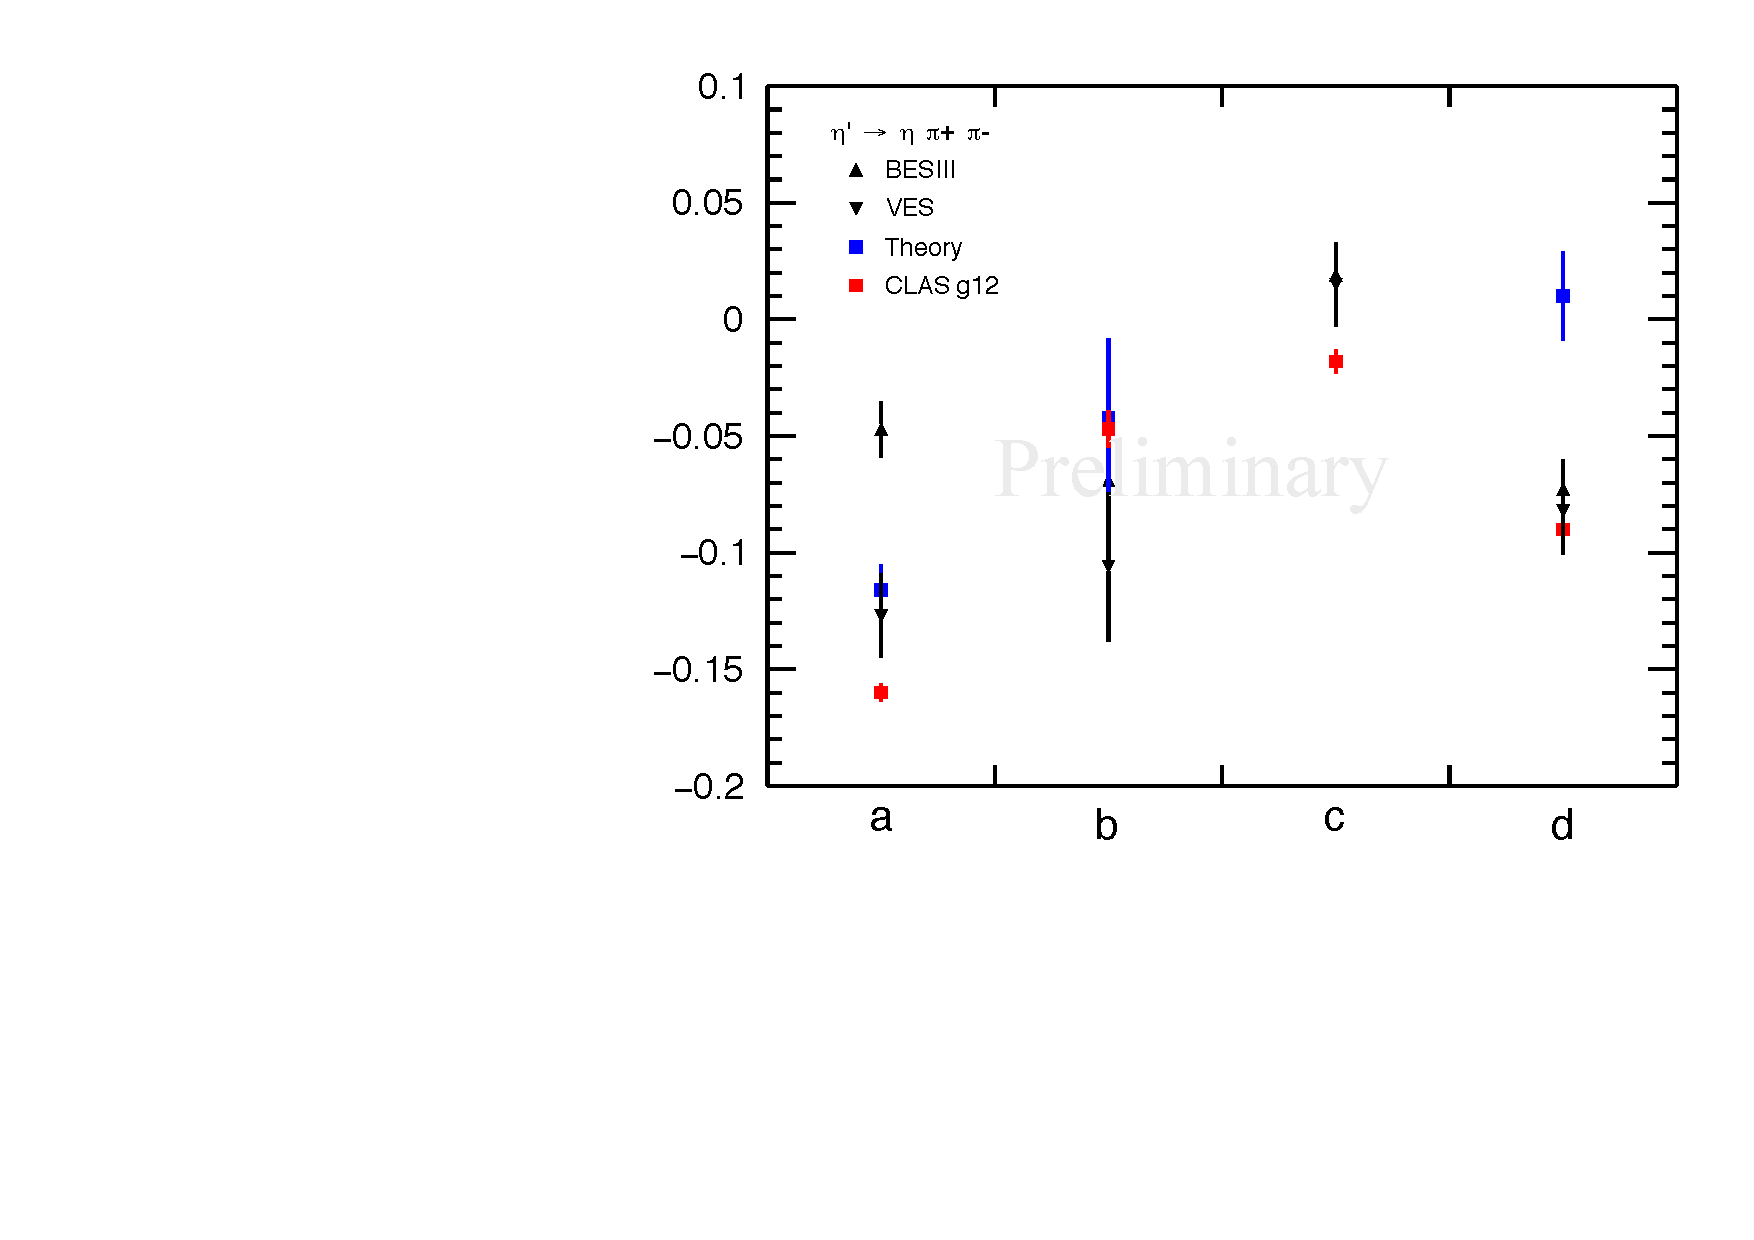
\includegraphics[width=10cm,height=5cm]{fit.pdf}
\end{center}

\begin{table}[!htb]
\centering
\begin{tabular}{|c|c|c|c|c|}
\hline
Parameter & {Theory [1]}           & VES [2]              & BESIII [3]          & { \textbf{Present Work}}   \\
\hline
a         & {-0.116 $\pm$ 0.011} & -0.127 $\pm$ 0.018 & -0.047 $\pm$ 0.012 & { \textbf{-0.160 $\pm$ 0.004}} \\
b         & {-0.042 $\pm$ 0.034} & -0.106 $\pm$ 0.032 & -0.069 $\pm$ 0.021 & { \textbf{-0.047 $\pm$ 0.008}} \\
c         & {...}              &{ 0.015 $\pm$ 0.018}  &{ 0.019 $\pm$ 0.012} & { \textbf{ -0.018 $\pm$ 0.005}} \\
d         & {+0.010 $\pm$ 0.019} & -0.082 $\pm$ 0.019 & -0.073 $\pm$ 0.013 & { \textbf{-0.090 $\pm$ 0.007}}  \\
\hline
$\frac{\chi^{2}}{NDF}$      &                                         & $\frac{129.3}{114}$ = 1.13                 & $\frac{504}{476}$ = 1.05                 & {$\frac{291}{97}$ = 3} \\
\hline
\end{tabular}
\end{table} 

%\begin {itemize}
%item I am sudeep
%\item N_{n} is no. of $\eta^{\prime}$ $\rightarrow$ $\eta$ $\pi^{+}$ $\pi^{-}$ events in the $n^{th}$ DP bin.
%\item $\epsilon_{n,m}$ is acceptance with smearing matrix, ie.  it gives acceptance of $m^{th}$ bin when events are generated in n$^{th}$ bin.
%\item $N_{theory,m}$ = $\int_{Boundary}$ A(1 + aY + bY^2 + cX + d X^2) dX dY
%\item $\sigma_{n}$ is the error associated with $n^{th}$ DP bin.
%\end{itemize}
